\documentclass{article}

\usepackage{amsmath, amsthm, amssymb, amsfonts}
\usepackage{thmtools}
\usepackage{graphicx}
\usepackage{setspace}
\usepackage{geometry}
\usepackage{float}
\usepackage[colorlinks=true, linkcolor=Blue]{hyperref}
\usepackage{cancel}
\usepackage[utf8]{inputenc}
\usepackage[english]{babel}
\usepackage{framed}
\usepackage[dvipsnames]{xcolor}
\usepackage{tcolorbox}
\usepackage{empheq}
\newtcolorbox{mymathbox}[1][]{colback=white, sharp corners, #1}
\usepackage{witharrows}

\author{Mauro Patimo}
\title{AERSP 508 Lecture 25}
\begin{document}
\maketitle
We can determine the drag coefficient by starting with the skin friction coefficient and integrating it over the surface of the body. Since the drag will be applied on both sides of the object, we need to multiply it by 2:
\begin{equation}
    C_D=\frac{2}{L}\int_0^L0.664\sqrt{\frac{\nu}{u_e}}x^{-\frac{1}{2}}dx
\end{equation}
where $u_e$ is the velocity at the end of the plate. The integral can be solved analytically and the result is:
\begin{equation}
    C_D=1.328\sqrt{\frac{\nu}{u_eL}}
\end{equation}
The Blasius profile is observed to approach the edge velocity asymptotically, so we cannot ascribe a definite thickness to the BL. However, we can define the boundary layer thickness as the distance from the wall where the velocity is 99\% of the edge velocity. This is also where $f'(\eta)=0.99$, which is $\eta=3.74$.
This gives 
\begin{equation}
    \delta=\delta_{99}=5.29\sqrt{\frac{\nu x}{u_e}}
\end{equation}
The Blasius similarity solution may be extended to flows over wedges, which are geometrically self-similar. The wedge angle is $\theta$ and the flow is assumed to be two-dimensional. The wedge is assumed to be semi-infinite, so the flow is assumed to be uniform at infinity. The velocity is $U_e=U_ox^m$. The angle of the wedge is $\pi\beta$. Beta is deined in the following way:
\begin{equation}
    \beta=\frac{2m}{1+m}
\end{equation}
$m$ can then be used to describe the angle of the wedge. We can find a relation between $m$ and the pressure gradient with Bernoulli's equation:
\begin{equation}
    \frac{1}{\rho}\frac{dP}{dx}=-U_e\frac{dU_e}{dx}=\frac{mU_e^2}{x} \footnote{$\frac{dU_e}{dx}=\frac{mU_e}{x}$ because $U_e=U_ox^m$}
\end{equation}
From this we can determine if the pressure gradient is favorable or adverse. If $m<0$, the pressure gradient is favorable, and if $m>0$, the pressure gradient is adverse. If $m=0$, the pressure gradient is zero. An example of a favorable pressure gradient is the flow encountering an obstacle, while an example of an adverse pressure gradient is a pipe increasing in diameter. As shown in Fig. \ref{fig:Wedges Examples}.
\begin{figure}
    \centering
    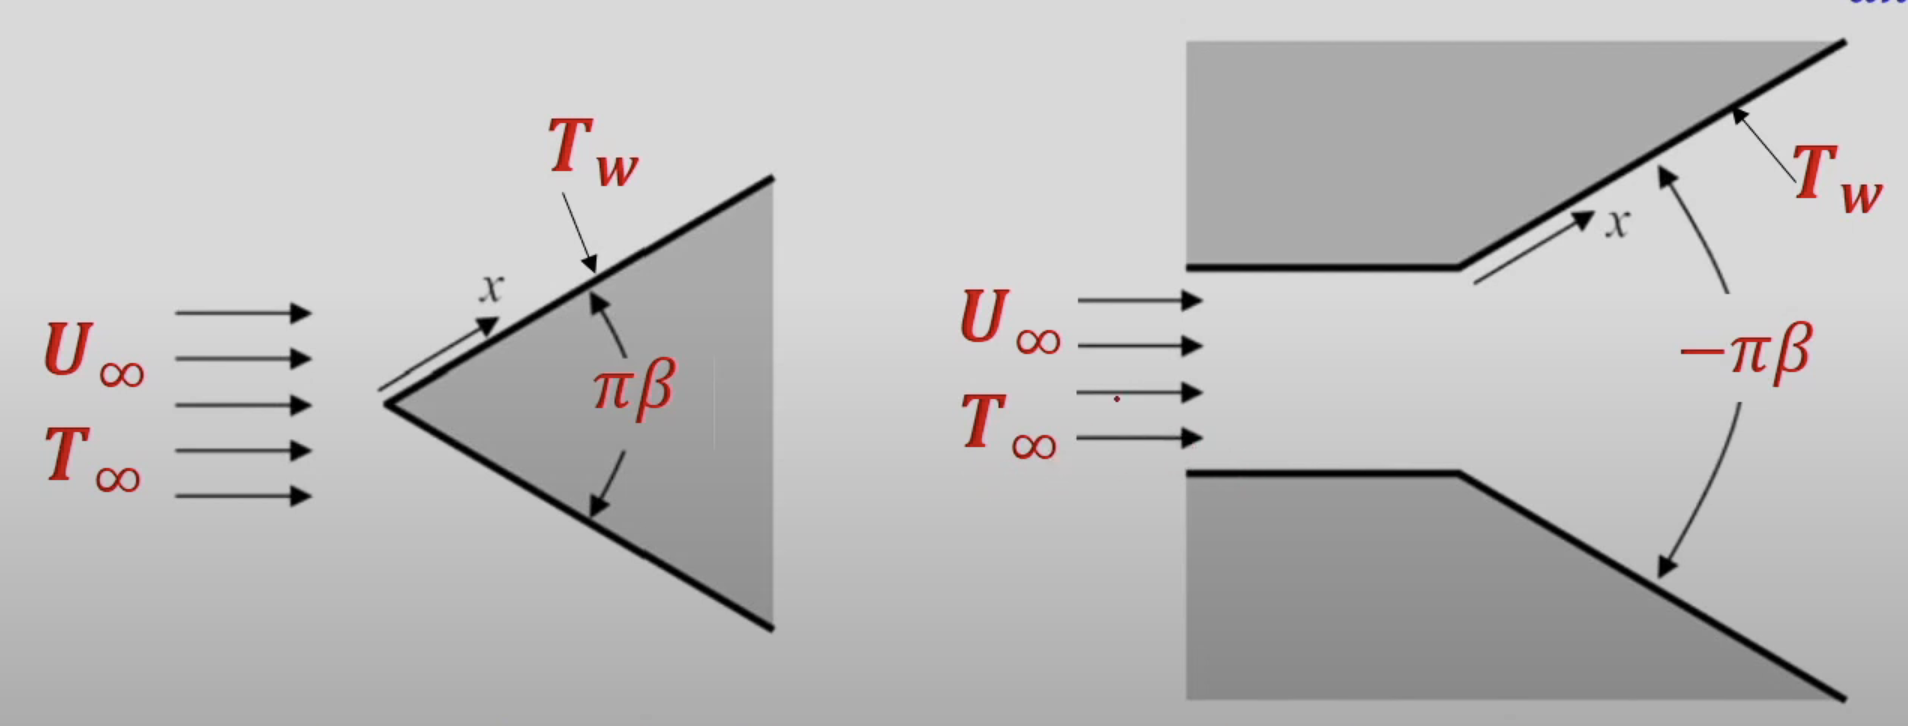
\includegraphics[width=\textwidth]{Wedges Examples.png}
    \caption{Examples of favorable and adverse pressure gradients. In this case $T$ stand for the temperature of the flow, but it is kept constant so it doesn't affect the flow.}
    \label{fig:Wedges Examples}
\end{figure}

\end{document}